\section{Deterministic multitasking}

\subsection{Control and stabilization}

\frame {
  \frametitle{Control systems}
  \begin{itemize}
    \item Computers control platforms
    \item Platforms must be kept stable
      \pause
    \item Done via \alert{control loops} that implement \alert{control
      laws}
    \item Control laws are mathematical descriptions
    \item Always iterative
      \pause
      \begin{enumerate}
        \item Read sensors
        \item Calculate response
        \item Send output to actuators
      \end{enumerate}
  \end{itemize}
  \pause
  \begin{center}
    $\includegraphics[scale=1]{../figs/impulse}$
  \end{center}
}

\frame {
  \frametitle{How they're done}
  \begin{itemize}
    \item Almost always implemented with cyclic executives
    \item Results in \alert{synchronous reactive systems}
    \item MATLAB \simu and SCADE Suite are often used
    \item Deterministic execution, any two runs are
      \emph{exactly} same
    \item Predominant paradigm is data flow
    \item Periodic threads or synchronous blocks exchanging data
    \item All attendant disadvantages of cyclic/synchronous systems
  \end{itemize}
}

\frame {
  \frametitle{Doing it asynchronously}
  \begin{itemize}
    \item Why not do it with a process based runtime?
    \item Gives asynchronous system, but use periodic threads, right?
    \item Allows true sporadic threads in the system as well
      \pause
    \item \alert{Non-deterministic execution}
    \item No guarantee that two runs will be exactly the same
    \item Data dependancies broken, a key feature of control loops
    \item Non-determinism can occur due to sporadic threads
  \end{itemize}
  \pause
    \begin{center}
    $\includegraphics[scale=1.75]{../figs/det_breach_presentation}$
  \end{center}
}

\subsection{Ensuring determinism}

\frame {
  \frametitle{A protocol to ensure determinism}
  \begin{itemize}
    \item A solution exists: sacrifice freshness for determinism
    \item Take last sample from previous hyperperiod
    \item Removes non-determinism due to interlacing and preemption
  \end{itemize}
  \pause
  \begin{center}
    $\includegraphics[scale=1.75]{../figs/det_no_breach_presentation}$
  \end{center}
  \pause
  \begin{itemize}
    \item \textbf{Assumption:} the periods of both threads must be
      harmonic
  \end{itemize}
}

%\frame {
%  \frametitle{Implementing the protocol---Suboptimal solution}
%  \begin{itemize}
%    \item Double buffer for every data flow
%    \item Source$\to$\alert{back buffer}$\ldots$\alert{front
%      buffer}$\to$Destination
%    \item \alert{Protcol task}: back buffer$\to$ front buffer at
%      hyperperiod boundary
%  \end{itemize}
%  \pause
%  \begin{center}
%    $\includegraphics[scale=1.75]{../figs/protocol_task}$
%  \end{center}
%}

\frame {
  \frametitle{Implementing the protocol}
  \begin{itemize}
    \item Double buffer for every data flow
    \item Source$\to$\alert{back buffer}$\ldots$\alert{front
      buffer}$\to$Destination
    \item \alert{Protcol task}: back buffer$\to$ front buffer at
      hyperperiod boundary
      \pause
    \item System is hard real-time, some important assumptions
      \begin{itemize}
        \item Faster task$\implies$higher priority, will execute
          first
        \item Source \& destination tasks periodic, $T_{long} =
          r\times T_{short}$
        \item Source thread writes at each job into the data flow
        \item Destination thread reads from data flow at each job
      \end{itemize}
    \item With assumptions, protocol handling goes into PO procedures
  \end{itemize}
}

\frame {
  \frametitle{DBX (Deterministic Bridge Exchangers)}
  \begin{itemize}
    \item Protected objects, like exchangers
    \item But with specialized \texttt{Get\_Value} and
      \texttt{Set\_Value} procedures
  \end{itemize}
  \pause
  \textbf{Stepper exchanger}
  \begin{itemize}
    \item Implements data flow from fast to slow task
    \item Buffer handling logic is in \texttt{Set\_Value}
    \item Copies buffer at every $r^{th}$ invocation, where
      $r=T_{long}/T_{short}$
  \end{itemize}
  \pause
  \textbf{Stagger exchanger}
  \begin{itemize}
    \item Implements data flow from slow to fast task
    \item Buffer handling logic is in \texttt{Get\_Value}
    \item Copies buffer at \emph{every} invocation, returns front
      buffer
  \end{itemize}
}

\subsection{Integration into AADL and tooling}

\frame {
  \frametitle{Automatic generation}
  \begin{itemize}
    \item Tedious \emph{and} error-prone to write these connectors
    \item AADL property defined for data port connections,
      \texttt{Is\_DBX}
    \item If \alert{\texttt{Is\_DBX}$\implies$\texttt{True}} then
      appropriate DBX generated
  \end{itemize}
  \pause
  \begin{center}
    $\includegraphics[scale=1.6]{../figs/transform_presentation}$
  \end{center}

}

\subsection{Verification}

\frame {
  \frametitle{Why verify}
  \begin{itemize}
    \item Safety-critical software, control systems need certification
    \item Certification usually done via tests
    \item Tests are expensive and time consuming
    \item Verification is another method to certify software
    \item Evidence exists that both methods are useful (MoD report)
  \end{itemize}
}

\frame {
  \frametitle{LOTOS}
  \begin{itemize}
    \item LOTOS is a process algebra
    \item Describes ``processes'' that engage in
      ``actions'' over ``gates''
    \item Processes composed together to form processes and systems
    \item Widely used method to model and verify distributed systems
    \item Creates a labelled transition system from the composed parts
    \item Carries out state space exploration
    \item ARC generates LOTOS code for each thread in a DBX connection
    \item Also generates LOTOS code for each DBX connector
    \item Composition gives LTS for system
  \end{itemize}
}

\frame {
  \frametitle{Example LTS}
  \begin{center}
    $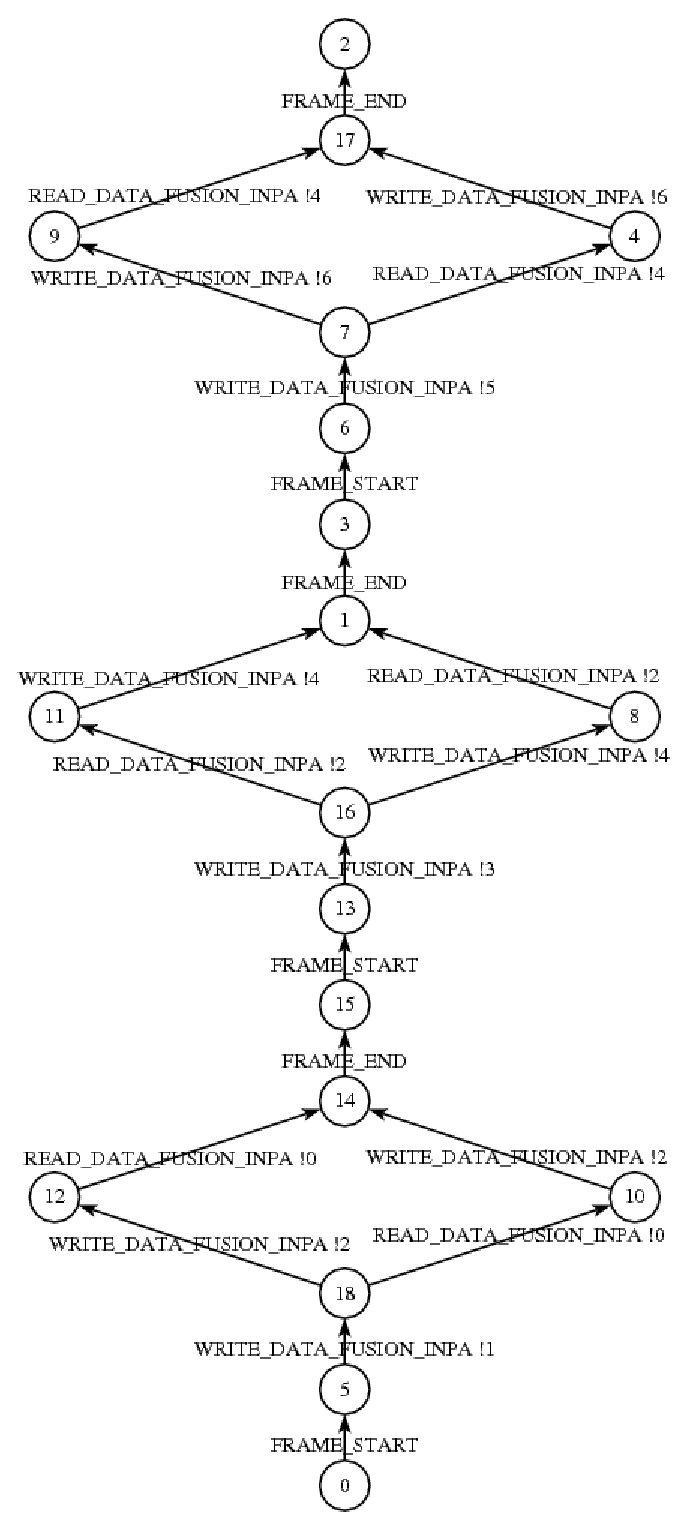
\includegraphics[angle=90, scale=0.4]{../figs/lotos_lts_ex1}$
  \end{center}
}

\subsection{Higher-order DBX}

\frame {
  \frametitle{Higher order sampling}
  \textbf{Higher order DBX}
  \begin{itemize}
    \item Same principle as simple DBX
    \item Instead of double buffer, have a queue
    \item Instead of buffer copy, ``promote'' members of the queue
    \item New AADL property, \texttt{Hyperperiod\_Age}
  \end{itemize}
  \pause
  \begin{center}
    $\includegraphics[scale=0.75]{../figs/ho-exch}$
  \end{center}
}  

\frame {
  \frametitle{Possible use}
  Consider the second-order filter
  \begin{displaymath}
    H(z) = \frac{az^2 + bz + c}{z^2 + dz + e}
  \end{displaymath}
  \pause
  Output can be written as
  \begin{displaymath}
    y = ax + (bx-dy)z^{-1} + (cx-ey)z^{-2}
  \end{displaymath}
  \pause
  Cannot be implemented using regular DBX connector

  Implemented as an AADL design as
  \begin{center}
    $\includegraphics[scale=0.7]{../figs/ho-example}$
  \end{center}
}

